\par Para este experimento evaluamos la red inalámbrica de los laboratorios del DC.

\subsubsection{Fuente $S$}

\par A continuación podemos ver la fuente $S$ propuesta, modelada con los resultados del experimento: \\

\begin{tabular}{ | c | c | c |}
    \hline
    Mensaje & Probabilidad & Información [bits] \\
    \hline
    \textit{Unicast} & 0.773 & 0.371 \\
    \hline
    \textit{Broadcast} & 0.227 & 2.141 \\
    \hline
\end{tabular} \\

\par Entropía de la fuente: 0.772 bits. Entropía máxima: 1 bit.

\par Observamos que la entropía de la fuente es menor que la máxima, ya que las transmisiones \textit{unicast} son casi 3 veces más probables que las \textit{broadcast}.
Esto nos provee una cota inferior para el \textit{overhead} impuesto por los protocolos de control: al menos 22.7\% de los frames no transmiten datos.

\subsubsection{Estructura de la red en base a los paquetes ARP}

\par En las figuras \ref{ARPDC-sinColapsar} y \ref{ARPDC} se pueden ver los grafos\footnote{Ambos grafos representan la misma red. Sin embargo, el tamaño del grafo \ref{ARPDC-sinColapsar} puede dificultar un análisis detallado, por lo que en la figura \ref{ARPDC} colapsamos ciertos nodos con iguales vecinos (que se muestran en rojo). Mantuvimos el grafo original ya que una mirada rápida ofrece más información concerniente a la topología de la red.} de la red subyacente de mensajes ARP.

\begin{figure*}[ht]
    \centering
    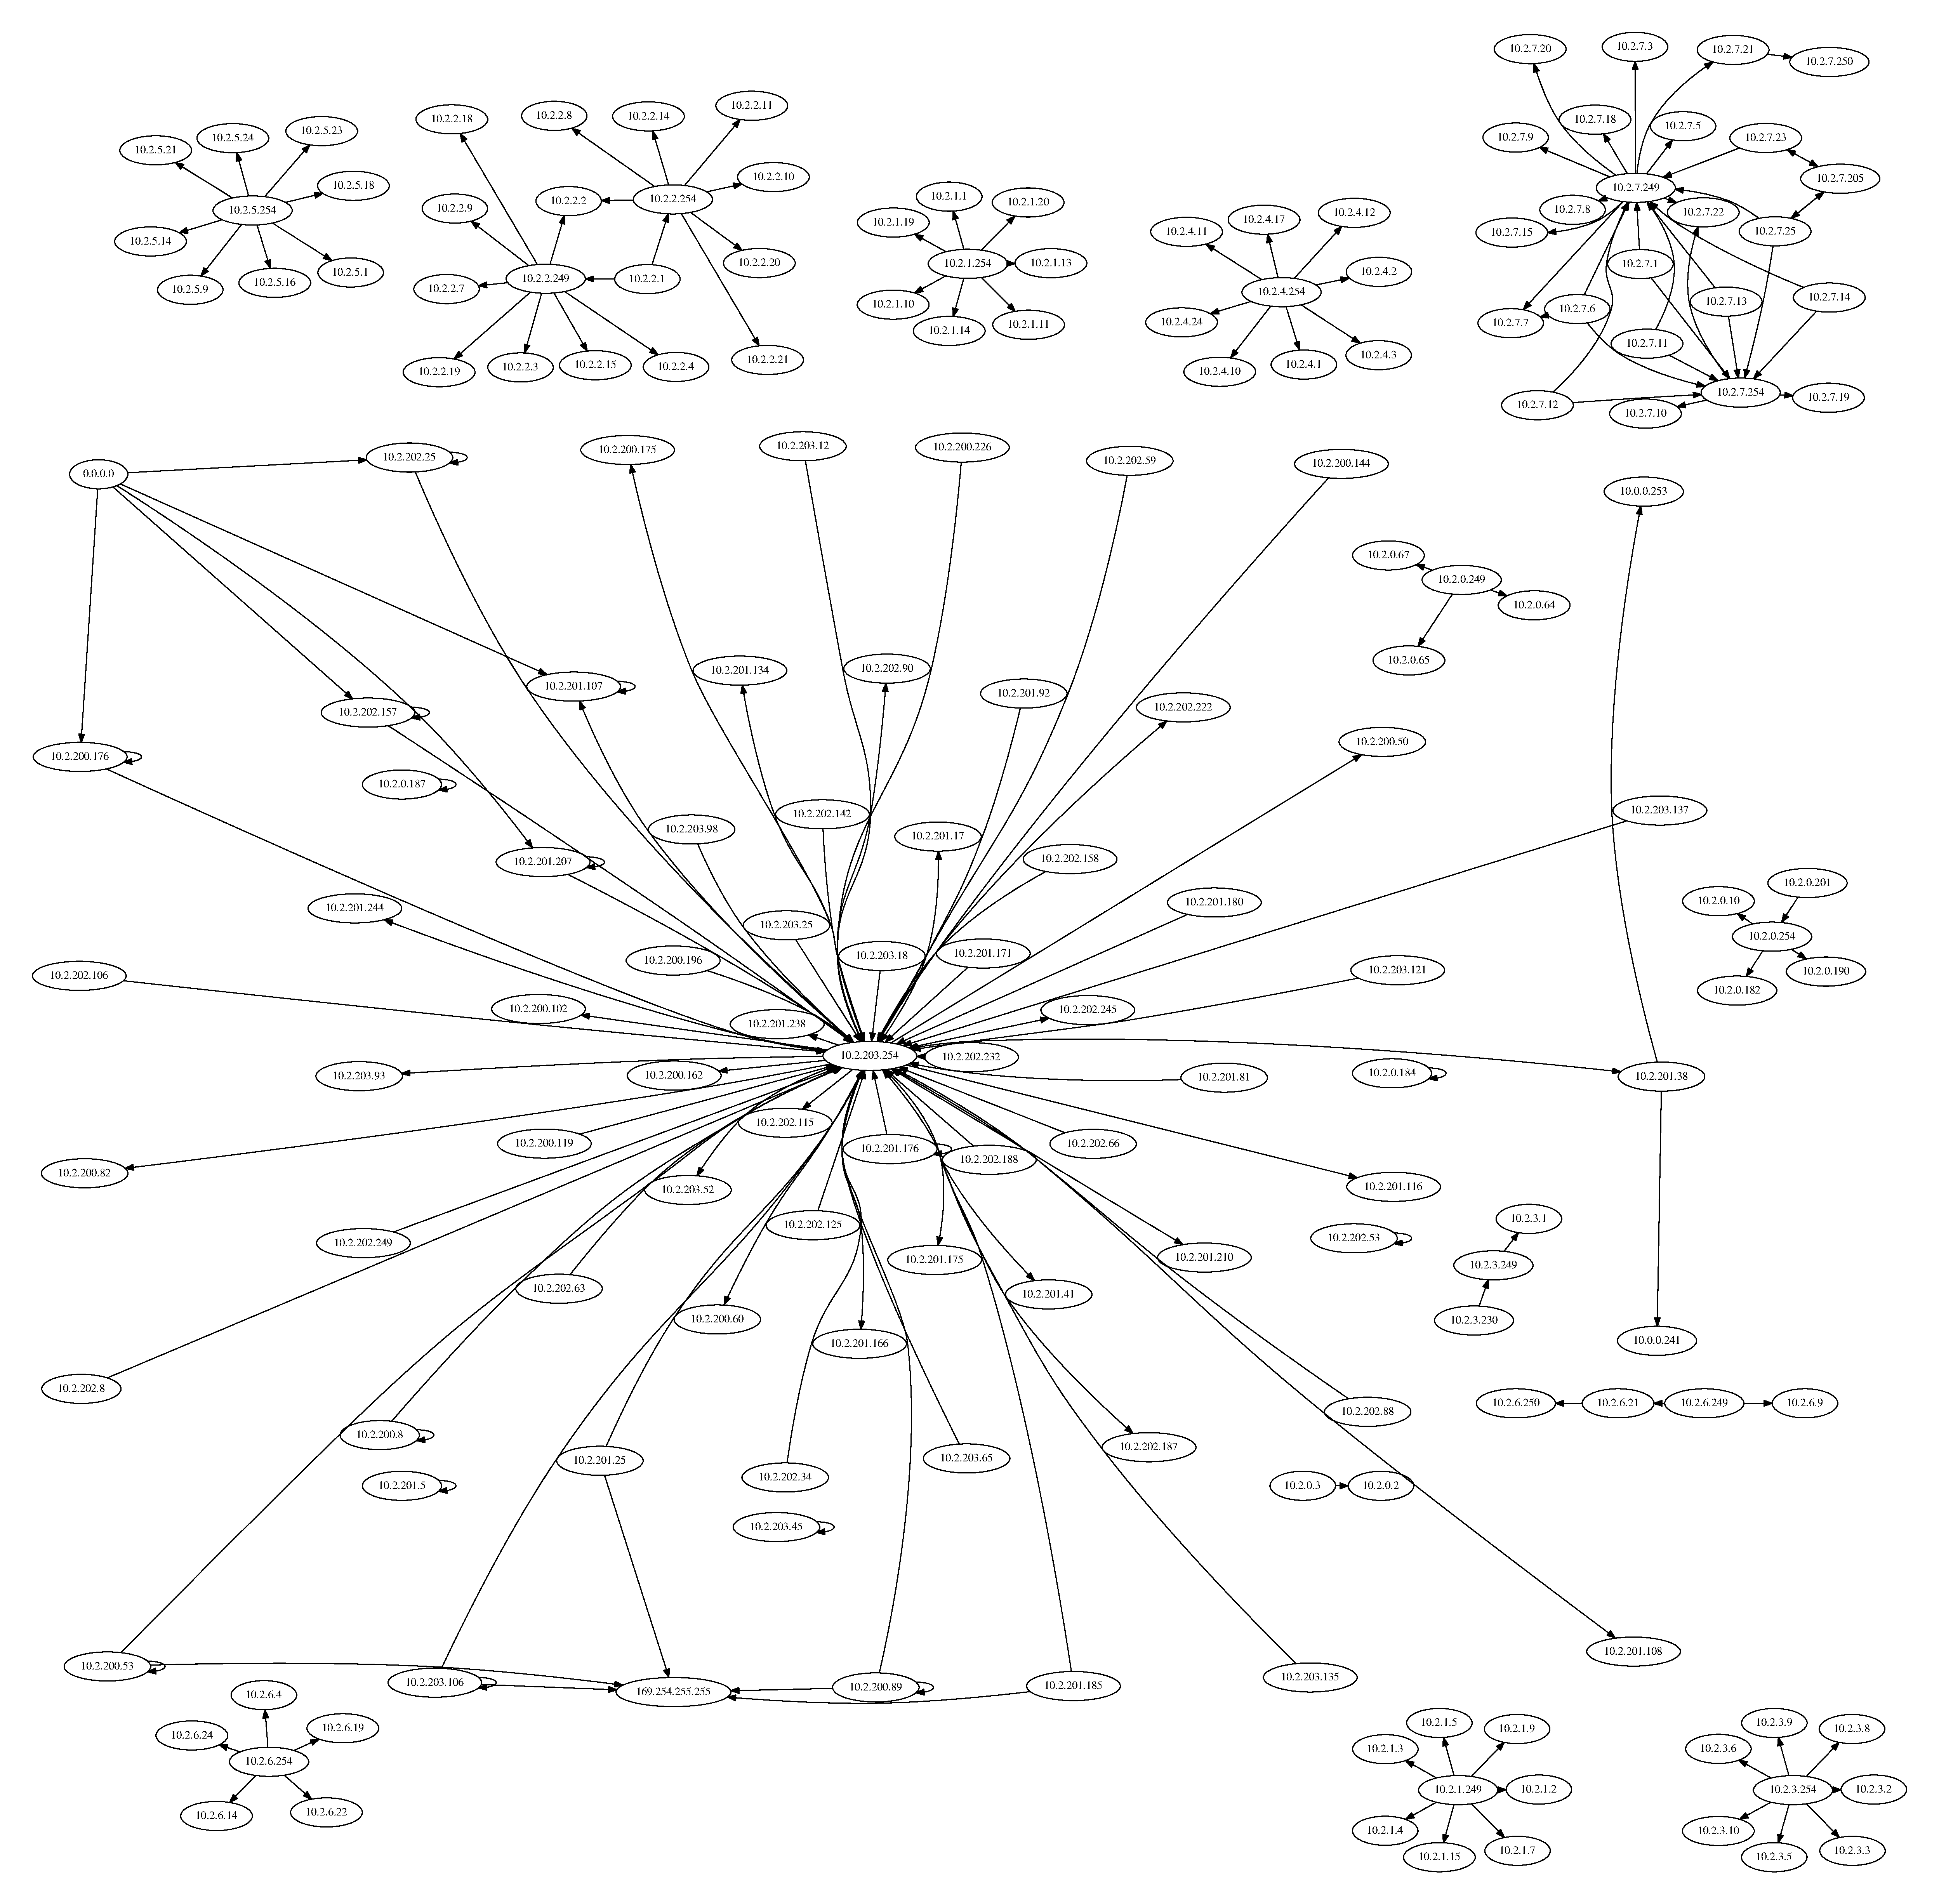
\includegraphics[width=0.9\textwidth]{figuras/ciudad_10_grafoSinColapsar.pdf}
    \caption{Grafo de la red subyacente de mensajes ARP en el experimento 1, sin colapsar nodos .}\label{ARPDC-sinColapsar}
\end{figure*}

\begin{figure*}[ht]
    \centering
    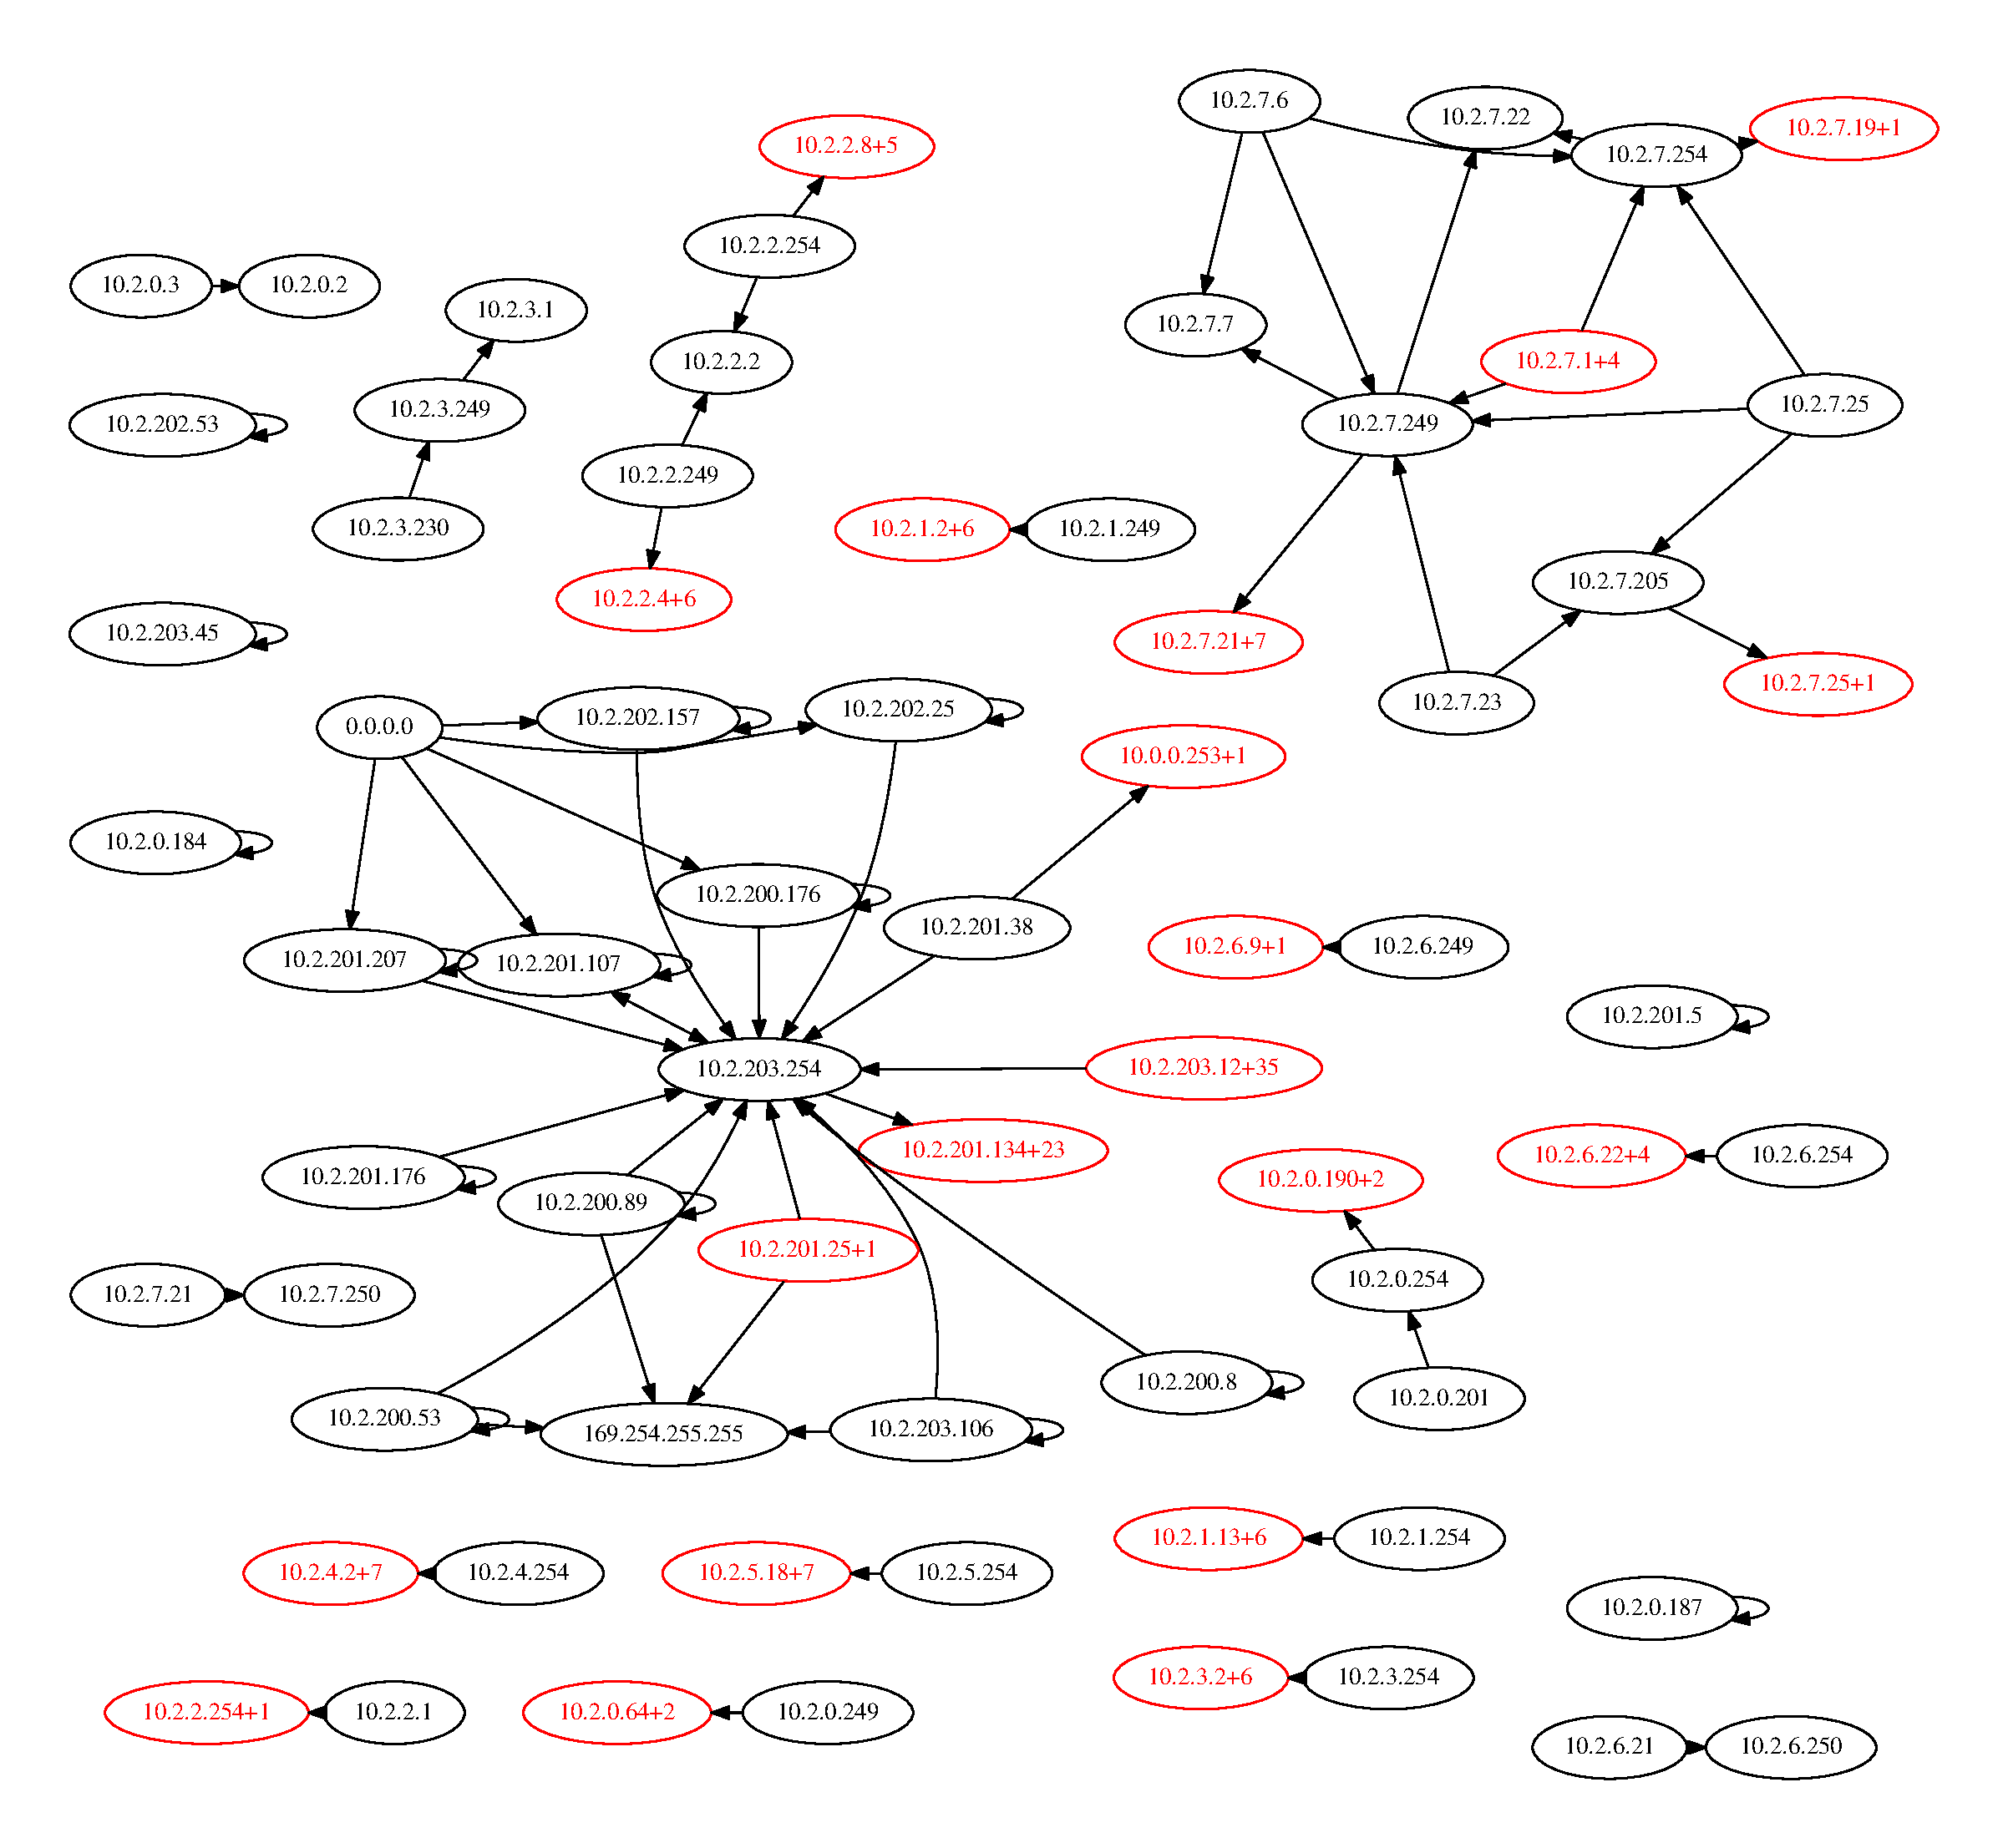
\includegraphics[width=0.9\textwidth]{figuras/ciudad_10_grafo.pdf}
    \caption{Grafo de la red subyacente de mensajes ARP en el experimento 1, colapsando nodos.}\label{ARPDC}
\end{figure*}

\par Las direcciones IP de la red son de la forma 10.2.X.Y, con una sola excepción que mencionaremos más adelante.
Éstas son direcciones IP privadas\footnote{Todo el rango 10.0.0.0-10.255.255.255 es privado.}.

\par La red se presenta altamente fragmentada; el grafo posee múltiples componentes conexas.
Adicionalmente, vemos repetido un patrón entre varias de estas componentes: un nodo central, con una dirección IP de la forma 10.2.X.254 o 10.2.X.249, que envía paquetes a múltiples hojas\footnote{Se presenta una estructura de estrella, o cercana.}.
Esta estructura es consistente con el comportamiento esperado de Default Gateways. 

\par Hay un nodo claramente destacado en la red, el de dirección IP 10.2.203.254, que tanto envía como recibe paquetes de un gran número de hojas.

\par Se advierten diversas anomalías: en primer lugar, loops en el grafo, que como mencionamos previamente, se deben a \textit{gratuitous ARPs}; en segundo lugar, la dirección 0.0.0.0 se hace presente en el grafo, siempre como origen, lo que ejemplifica \textit{ARP probing}; finalmente, una única IP que no comienza con 10.2, la 169.254.255.255.
El rango 169.254.0.0-169.254.255.255 está reservado; se asigna cuando un dispositivo no tiene IP estática, y el protocolo dinámico\footnote{DHCP siendo actualmente el más común.} utilizado falla.

\subsubsection{Fuente $S_1$}

\par En la tabla \ref{tab1SinRSinA} podemos ver la información de ciertos\footnote{La alta cantidad de nodos dificulta seriamente la presentación de estos resultados, tanto en forma de gráficos como de tablas.
En las siguientes tablas listaremos todos los nodos distinguidos, y los nodos que, en base a ciertos criterios, nos parecieron destacados pero la fuente no distinguió.} mensajes de la fuente $S_1$, sin paquetes repetidos y tomando sólo el \textit{Sender's Protocol Address} de los paquetes.

\par La entropía de la fuente es de 5.61 bits, siendo la máxima 32 bits. 

\begin{table}[t]
    \centering
    \begin{tabular}{ | c | c | c | l |}
        \hline
        Mensaje & Información [bits] & Distinguido?\\
        \hline
        10.2.3.249 & 7.58 & No \\ %
        \hline
        10.2.202.249 & 7.58 & No \\ %
        \hline
        10.2.6.249 & 6.58 & No \\ %
        \hline
        10.2.7.254 & 6.00 & No \\
        \hline
        10.2.0.254 & 6.00 & No \\
        \hline
        10.2.0.249 & 6.00 & No \\
        \hline
        10.2.6.254 & 5.26 & Sí \\
        \hline
        10.2.1.254 & 4.78 & Sí \\
        \hline
        10.2.1.249 & 4.78 & Sí \\
        \hline
        10.2.3.254 & 4.78 & Sí \\
        \hline
        10.2.2.254 & 4.78 & Sí \\
        \hline
        10.2.2.249 & 4.58 & Sí \\
        \hline
        10.2.4.254 & 4.58 & Sí \\
        \hline
        10.2.5.254 & 4.58 & Sí \\
        \hline
        10.2.7.249 & 4.26 & Sí \\
        \hline
        10.2.203.254 & 2.94 & Sí \\
        \hline
    \end{tabular} 
    \caption{Información de los nodos de la fuente $S_1$ en el experimento 1, sin tomar paquetes repetidos y considerando como mensaje la ocurrencia de una IP en el campo \textit{Sender's Protocol Address} de un paquete ARP \textit{who-has}.}
    \label{tab1SinRSinA}
\end{table} 

\par Vemos que no se producen falsos positivos: todos los nodos que la fuente distingue son los que destacamos previamente, con direcciones IP de la forma 10.2.X.249 o 10.2.X.254.
Sin embargo, vemos ciertos potenciales falsos negativos.

\par Los tres primeros, es decir el 3.249, el 202.249 y el 6.249\footnote{Obviando de las direcciones el 10.2. inicial.}, si bien sus IPs son de la forma destacada, no parecen exhibir el comportamiento de los otros\footnote{En el grafo no se presentan en el centro de una estructura de estrella o similar.} ni actuar como Default Gateways.
Por ende, concluimos que no clasificarlos como distinguidos no es una falencia de la fuente.

\par Sin embargo los tres restantes, el 7.254, el 0.249 y el 0.254, presentan el comportamiento mencionado y exhiben la estructura de estrella, pero no son clasificados como distinguidos.
En el caso del 0.249, esto se debe a que no tiene suficientes vecinos, por lo que su información es relativamente baja; es posible que esta falencia pueda ser subsanada al considerar paquetes repetidos.
Por otro lado, el 0.254 y el 7.254, tienen más vecinos pero varios de éstos presentan ejes en el otro sentido que el aceptado por la fuente\footnote{Es decir, este nodo es el destino de varios paquetes ARP, no el origen.}; es posible que este error sea resuelto aceptando ejes en ambas direcciones.

\par En la tabla \ref{tab1A} podemos ver la información de ciertos mensajes de la fuente $S_1$, sin paquetes repetidos y tomando tanto el \textit{Sender's Protocol Address} como el \textit{Target Protocol Address} de los paquetes.

\begin{table}[t]
    \centering
    \begin{tabular}{ | c | c | c | l |}
        \hline
        Mensaje & Información [bits] & Distinguido?\\
\hline
10.2.202.249 & 8.55 & No \\
\hline
10.2.3.249 & 7.55 & No \\
\hline
10.2.6.249 & 7.55 & No \\
\hline
10.2.0.249 & 6.96 & No \\
\hline
10.2.0.254 & 6.55 & No \\
\hline
10.2.6.254 & 6.22 & Sí \\
\hline
169.254.255.255 & 6.22 & Sí \\
\hline
10.2.3.254 & 5.74 & Sí \\
\hline
10.2.1.249 & 5.74 & Sí \\
\hline
10.2.1.254 & 5.74 & Sí \\
\hline
10.2.5.254 & 5.55 & Sí \\
\hline
10.2.4.254 & 5.55 & Sí \\
\hline
10.2.2.254 & 5.55 & Sí \\
\hline
10.2.2.249 & 5.38 & Sí \\
\hline
10.2.7.254 & 5.22 & Sí \\
\hline
10.2.7.249 & 4.38 & Sí \\
\hline
10.2.203.254 & 2.34 & Sí \\
\hline
    \end{tabular} 
    \caption{Información de los nodos de la fuente $S_1$ en el experimento 1, sin tomar paquetes repetidos y considerando como mensaje la ocurrencia de una IP tanto en el campo \textit{Sender's Protocol Address} como en el \textit{Target Protocol Address} de un paquete ARP \textit{who-has}.}
    \label{tab1A}
\end{table} 

\par La entropía de la fuente es de 6.28 bits, siendo la máxima 32 bits. 
Cabe destacar que la entropía es mayor que la de la fuente previa.
Muchos paquetes son enviados por un nodo destacado a direcciones que no aparecen nuevamente; la fuente previa sólo cuenta al nodo destacado, que al aparecer múltiples veces provee poca informacion, mientras que esta fuente cuenta también al nodo más raro, cuya información es más alta.

\par Vemos que uno de los falsos negativos que habíamos mencionado, el 7.254, es considerado distinguido en esta nueva fuente.
Se presenta otro nuevo nodo como distinguido: el 169.254.255.255. 
Previamente habíamos mencionado que ésta era una IP reservada con características específicas; no es absurdo considerarla destacada. 
Sin embargo, si la intención es que todo nodo destacado sea un Default Gateway, esto nos muestra que se deben eliminar ciertos rangos de direcciones particulares.

\par En la tabla \ref{tab1R} podemos ver la información de ciertos mensajes de la fuente $S_1$, con paquetes repetidos y tomando sólo el \textit{Sender's Protocol Address} de los paquetes.

\begin{table}[t]
    \centering
    \begin{tabular}{ | c | c | c | l |}
        \hline
        Mensaje & Información [bits] & Distinguido?\\
\hline
10.2.3.249 & 9.63 & No \\
\hline
10.2.202.249 & 9.63 & No \\
\hline
10.2.6.249 & 8.63 & No \\
\hline
10.2.7.254 & 7.63 & No \\
\hline
10.2.1.254 & 6.63 & No \\
\hline
10.2.0.254 & 6.63 & No \\
\hline
10.2.6.254 & 6.63 & No \\
\hline
10.2.2.254 & 6.46 & No \\
\hline
10.2.2.249 & 6.17 & No \\
\hline
10.2.5.254 & 6.04 & No \\
\hline
10.2.1.249 & 5.93 & No \\
\hline
10.2.4.254 & 5.82 & No \\
\hline
10.2.7.249 & 5.82 & No \\
\hline
10.2.3.254 & 5.54 & No \\
\hline
10.2.200.144 & 4.72 & Sí \\
\hline
10.2.200.176 & 4.68 & Sí \\
\hline
10.2.7.12 & 4.46 & Sí \\
\hline
10.2.7.25 & 4.42 & Sí \\
\hline
10.2.7.14 & 4.38 & Sí \\
\hline
10.2.2.1 & 4.27 & Sí \\
\hline
10.2.7.11 & 4.24 & Sí \\
\hline
10.2.203.254 & 4.07 & Sí \\
\hline
10.2.7.6 & 4.07 & Sí \\
\hline
10.2.7.1 & 4.07 & Sí \\
\hline
10.2.7.13 & 3.99 & Sí \\
\hline
10.2.0.249 & 3.82 & Sí \\
\hline
    \end{tabular} 
    \caption{Información de los nodos de la fuente $S_1$ en el experimento 1, tomando paquetes repetidos y considerando como mensaje la ocurrencia de una IP en el campo \textit{Sender's Protocol Address} de un paquete ARP \textit{who-has}.}
    \label{tab1R}
\end{table} 

\par Entropía de la fuente: 5.20 bits. Entropía máxima: 32 bits.

\par Los resultados presentan una extrema cantidad de falsos positivos y negativos, por lo que concluimos que esta fuente no sirve para nuestros propósitos.

\par Debido a la mayor entropía y a la menor cantidad de falsos negativos de la fuente sin repetidos y con origen y destino, concluimos que ésta es preferible, al menos en las condiciones de este experimento.
